
\section{SEIRS modelling with mixing matrices}

Starting from the 1-community SEIRS model, 

\begin{figure}[H]
\centering
\tikzstyle{compartment}=[circle, draw, thick, inner sep=0pt, minimum size=7mm]
\tikzstyle{pointto}=[->,shorten >=1pt,>=stealth,semithick]
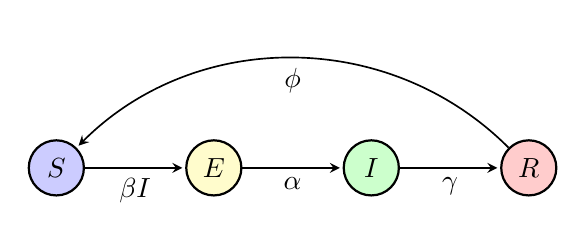
\begin{tikzpicture}
\node[compartment, fill=blue!20]  (S) at (0,0) {$S$};  % inner sep=6pt, 
\node[compartment, fill=yellow!20](E) at (2,0) {$E$};  % inner sep=6pt, 
\node[compartment, fill=green!20] (I) at (4,0) {$I$};  % inner sep=6pt, 
\node[compartment, fill=red!20]   (R) at (6,0) {$R$};  % inner sep=6pt, 
% \node[compartment](Q) at (4,-1) {Q}; % inner sep=6pt, 
\draw[pointto] (S) to node[below] {$\beta I$} (E);
\draw[pointto] (E) to node[below] {$\alpha$} (I);
\draw[pointto] (I) to node[below] {$\gamma$} (R);
\draw[pointto] (R) to[out=135, in=45] node[below] {$\phi$} (S);
\end{tikzpicture}

\end{figure}

the following diff equations can be set up:

\begin{align*}
\dv{t}S(t) =& - \frac{1}{N} \beta I(t) S(t) + \phi R \\
\dv{t}E(t) =& \frac{1}{N} \beta I(t)S(t) - \alpha E(t) \\
\dv{t}I(t) =& \alpha E(t) - \gamma I(t) \\
\dv{t}R(t) =& \gamma I(t) - \phi R
\end{align*}

where $\alpha$ is reciprocal incubation time,
$\beta$ is reciprocal time between contact,
$\gamma$ is reciprocal recovery time.
% and $\eta$ is efficiancy of infection (the proportion of exposed population becoming vectors of the diease).
Note that we here assume a consant population:

\begin{align*}
S(t) + E(t) + I(t) + R(t) = N \quad , \quad \forall t \in \left[ 0, \infty \right[ %\\
% \dv{t} \left( S(t) + E(t) + I(t) + R(t) \right) = 0
\end{align*}
this can now be normalized wrt. the population size $N$, to get dimentionless populations, and to eliminate the factor $N$ from the couple diff equations.
This model is for one homogenous population, and so to refine it, we now consider a modified model in which wh have several different communities\footnote{the communities we consider here are different age groups.}, all with their separate evolution system, such that the population in each community, is constant:

\begin{align*}
\dv{t}S_{i}(t) =& - \frac{1}{N_{i}} \beta I^{M}_{i}(t) S_{i}(t) + \phi R \\
\dv{t}E_{i}(t) =& \frac{1}{N_{i}} \beta I^{M}_{i}(t)S_{i}(t) - \alpha E_{i}(t) \\
\dv{t}I_{i}(t) =& \alpha E_{i}(t) - \gamma I_{i}(t) \\
\dv{t}R_{i}(t) =& \gamma I_{i}(t) - \phi R
\end{align*}

where in this model, the rate of exposiure is determined by the new quantity $I_{T}(t)$ that constitute the wheigted proprtion of the infectious population, given as:

\begin{align*}
I^{M}_{j}(t) = \sum_{f}\sum_{i}w^{f}_{j}(c^{f}_{ij})^{T}I_{i}(t)
\end{align*}

where the indices $i,j$ indicates the different age groups, and the index $f$, indicates the \textit{form of transmition}\footnote{or rather the context/sitution/type/incident. pick the one you like best.}, which can be picked as combinations from the folowing table:

\begin{table}[H]
\centering
\begin{tabular}{l | *{4}{c}}
\hline \\
Infection wheights & school (s) & work (w) & home (h) & other (o) \\
\hline \\
Physical (p) ($\times 1$)& 1 & 0.5 & 1 & 0.2 \\
Casual (c) ($\times 0.2$) & 0.2 & 0.1 & 0.2 & 0.04
\end{tabular}
\end{table}
This can now be vectorized as follows:

\begin{align*}
w_{i} = (w_{ps}, w_{pw}, w_{ph}, w_{po}, w_{cs}, w_{cw}, w_{ch}, w_{co})^{T}
\end{align*}

where the subscript indicates the product between the corresponding partial whaights, e.g. $w_{ph} = w_{p} w_{h}$.
Again, the populations agegroups copnpartments can be normalized wrt. the size of the agegroup, to eliminate the factor $N_{i}$ in the couple diff. eqn.s and get dimensionless sub-populations.

\begin{align*}
S_{i}(t) + E_{i}(t) + I_{i}(t) + R_{i}(t) = N_{i} = N p_{i} \quad , \quad \forall t \in \left[ 0, \infty \right[ \qquad \text{and} \qquad \sum_{i} p_{i} = 1
\end{align*}

The index indicating the different age groups is necessary if different stategies are emplored by different age groups e.g. the age group 0-9 yrs are allowed in school, while age group 10-19 yrs are not, which corresponds to setting the coorsponding school-wheights to zero for the latter group, but not the first.

With this in place, a script is made and the age-differentiated SEIR-model is is integrated numerically, using scipy-odeint package, with the following results:

\newpage

The weights described above, used in the scenario is:
\begin{table}[H]
\centering
\input{../meta/w_table_n.txt}
\end{table}

\begin{figure}[H]
\centering
\includegraphics[width = 0.75\textwidth]{../fig/SEIRS_total_population_mix_n.pdf}
\caption{
\protect\input{../fig/SEIRS_total_population_mix_figtext_n.txt} 
\label{fig:total_pop_mix_n}}
\end{figure}

\begin{figure}[H]
\centering
\begin{subfigure}{0.40\textwidth}
\includegraphics[width = \textwidth]{../fig/SEIRS_0-9_n.pdf}
\caption{\protect\input{../fig/SEIRS_0-9_figtext_n.txt}}
\end{subfigure}
\begin{subfigure}{0.40\textwidth}
\includegraphics[width = \textwidth]{../fig/SEIRS_10-19_n.pdf}
\caption{\protect\input{../fig/SEIRS_10-19_figtext_n.txt}}
\end{subfigure}
\begin{subfigure}{0.40\textwidth}
\includegraphics[width = \textwidth]{../fig/SEIRS_20-29_n.pdf}
\caption{\protect\input{../fig/SEIRS_20-29_figtext_n.txt}}
\end{subfigure}
\begin{subfigure}{0.40\textwidth}
\includegraphics[width = \textwidth]{../fig/SEIRS_30-39_n.pdf}
\caption{\protect\input{../fig/SEIRS_30-39_figtext_n.txt}}
\end{subfigure}
\begin{subfigure}{0.40\textwidth}
\includegraphics[width = \textwidth]{../fig/SEIRS_40-49_n.pdf}
\caption{\protect\input{../fig/SEIRS_40-49_figtext_n.txt}}
\end{subfigure}
\begin{subfigure}{0.40\textwidth}
\includegraphics[width = \textwidth]{../fig/SEIRS_50-59_n.pdf}
\caption{\protect\input{../fig/SEIRS_50-59_figtext_n.txt}}
\end{subfigure}
\begin{subfigure}{0.40\textwidth}
\includegraphics[width = \textwidth]{../fig/SEIRS_60-69_n.pdf}
\caption{\protect\input{../fig/SEIRS_60-69_figtext_n.txt}}
\end{subfigure}
\begin{subfigure}{0.40\textwidth}
\includegraphics[width = \textwidth]{../fig/SEIRS_70-_n.pdf}
\caption{\protect\input{../fig/SEIRS_70-_figtext_n.txt}}
\end{subfigure}
\end{figure}

% --

% \newpage
% 
% The weights described above, used in the scenario is:
% \begin{table}[H]
% \centering
% \input{../meta/w_table_q.txt}
% \end{table}
% 
% \begin{figure}[H]
% \centering
% \includegraphics[width = 0.75\textwidth]{../fig/SEIR_total_population_mix_q.pdf}
% \caption{
% \protect\input{../fig/SEIR_total_population_mix_figtext_q.txt} 
% \label{fig:total_pop_mix_q}}
% \end{figure}
% 
% \begin{figure}[H]
% \centering
% \begin{subfigure}{0.40\textwidth}
% \includegraphics[width = \textwidth]{../fig/SEIR_0-9_q.pdf}
% \caption{\protect\input{../fig/SEIR_0-9_figtext_q.txt}}
% \end{subfigure}
% \begin{subfigure}{0.40\textwidth}
% \includegraphics[width = \textwidth]{../fig/SEIR_10-19_q.pdf}
% \caption{\protect\input{../fig/SEIR_10-19_figtext_q.txt}}
% \end{subfigure}
% \begin{subfigure}{0.40\textwidth}
% \includegraphics[width = \textwidth]{../fig/SEIR_20-29_q.pdf}
% \caption{\protect\input{../fig/SEIR_20-29_figtext_q.txt}}
% \end{subfigure}
% \begin{subfigure}{0.40\textwidth}
% \includegraphics[width = \textwidth]{../fig/SEIR_30-39_q.pdf}
% \caption{\protect\input{../fig/SEIR_30-39_figtext_q.txt}}
% \end{subfigure}
% \begin{subfigure}{0.40\textwidth}
% \includegraphics[width = \textwidth]{../fig/SEIR_40-49_q.pdf}
% \caption{\protect\input{../fig/SEIR_40-49_figtext_q.txt}}
% \end{subfigure}
% \begin{subfigure}{0.40\textwidth}
% \includegraphics[width = \textwidth]{../fig/SEIR_50-59_q.pdf}
% \caption{\protect\input{../fig/SEIR_50-59_figtext_q.txt}}
% \end{subfigure}
% \begin{subfigure}{0.40\textwidth}
% \includegraphics[width = \textwidth]{../fig/SEIR_60-69_q.pdf}
% \caption{\protect\input{../fig/SEIR_60-69_figtext_q.txt}}
% \end{subfigure}
% \begin{subfigure}{0.40\textwidth}
% \includegraphics[width = \textwidth]{../fig/SEIR_70-_q.pdf}
% \caption{\protect\input{../fig/SEIR_70-_figtext_q.txt}}
% \end{subfigure}
% \end{figure}
